\section{Transitioning to Three Dimensions}
The move to 3D was slow, the jump from \emph{pygame} to a full blown physics simulation was a big leap and it came with its problems.

\subsection{CoppeliaSim and RLBench}

CoppeliaSim is a mostly open source simulation program that provides full access to its features through an educational license and RLBench \cite{james2019rlbenchrobotlearningbenchmark} is an in-house (Imperial) tool adapted to plug into CoppeliaSim through its python API interface, PyRep \cite{pyrep2020}. 

There are many tutorials online to help learn how CoppeliaSim operates and designing some scenes \todo[color=green]{maybe cite some stuff here, not necessary}. However, RLBench is a harder beast to tame. Although the system is very smart and it eliminates a lot of the required manual work before starting experimenting; it is quite old, plugs into version $4.1$ of CoppeliaSim from 2020. As well as its age, I had had some issues setting it up on my system. 

\subsection{Environment Issues}\todo[color=red]{this section might need shortening, 2 pages is a lot for this}
One of the first large-scale issues I'd face in this project came quite early in its lifespan. I would soon learn robotics development is mostly done on Linux based machines and the journey to getting everything working would be quite long.

\subsubsection{Windows Setup}
I do most development work on Windows and WSL (Windows Subsystem for Linux) \cite{microsoftWSL} and expecting this project to be memory and graphic power hungry, it made sense to set everything up on the Windows side. This caused a few issues with PyRep, mainly because PyRep expected to be running on Linux, and RLBench was having issues launching.

\subsubsection{WSL Setup}
I thought this wouldn't be a problem, as WSL version 2 has been pretty good with GUI applications running on Linux and thought I could run Coppelia on there and still access any GUI (Graphical User Interface) I might need while developing tasks and observing my robot.

The translation layer between the operating systems might cause some slowing but there shouldn't be any major issues. Upon configuring everything as the installation guide suggested in RLBench and PyRep repositories. I had few issues linking object files downloaded with CoppeliaSim into the PyRep layer. After spending a lot of time researching issues, and coming across some online threads with similar issues (in different applications, so nothing was immediately applicable) I decided WSL must have been the problem and decided to move onto the next logical step.
 
\subsubsection{Linux Virtual Machine}
I had previously used Ubuntu a lot and even my WSL instance was running Ubuntu. As RLBench suggested Debian based systems, and seeing the tutorials were done on Ubuntu, I created a Virtual Machine running it. After the entire setup process, I was finally able to get the instance running and finally managed to run one of the examples that gets downloaded when installing RLBench.

However, I got hit by another issues fairly quickly, the rendering of Virtual Box was definitely going through some sort of translation through Windows and the GPU adapter was not linking properly. So, everything was extremely sluggish, and running the non-primitive examples even crashed my virtual machine instances a few times. At this point I realised I had to settle for the real deal and got to partitioning by storage drive.

\subsubsection{Dual Booting}
I had some issues partitioning the drive Windows was already installed, so decided to get myself another drive I could boot Ubuntu from.

After running through the same setup steps and linking binaries, I was finally properly running RLBench. With one caveat, CoppeliaSim constantly complained that I was missing some video compression libraries; though seemed to work perfectly fine after installing them. It would always complain to me with a pop-up (see Figure \ref{fig:missing-libs}) but I found no issues with it during the project. There were other small annoyances like this throughout the entirety of the experimentation but finally I had everything working.

\begin{figure}[htpb] % htpb allows all placement
  \centering
  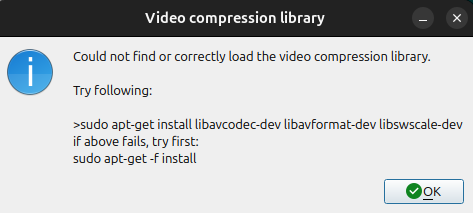
\includegraphics[scale=0.3]{assets/early-work/missing-libs.png}
  \caption{}\label{fig:missing-libs}
\end{figure}


\subsubsection{Side Note on Campus Machines}
I knew that a solution to all of my problems might have been using a machine at the labs. I thought an issue with that may have been that RLBench needs some binary linking and setting of system variables, which might have required more access rights and the troubleshooting wouldn't be as easy as doing it on my machine. 

However, the main reason I didn't try this is because my personal machine has appropriately powerful hardware for a machine learning project and wanted to take advantage of this. So jumping through all these steps took about an entire week, but was well worth it, as now I have a system that can run all these systems in a headed manner, meaning I can watch and observe the behaviours of my robot as it learns and explores its workspace, to possibly see its shortcomings and propose methods in eliminating them.

\subsection{Usability Issues}\todo{maybe combine this and the next PyBullet section under the Toolset Dilemma section, to shorten these here}
I had some instability issues mainly due to RLBench's age which is about 5 years old now. CoppeliaSim has moved on in some parts. However, PyRep didn't not work with any other version other than version $4.1$ (2020), CoppeliaSim is now at $4.9$ (2025) \cite{coppeliaSimManual}.
There was work being done on updating PyRep to version 4.6 \ref{pyrep460beta} last year, but I did not feel confident in using a beta build after all the issues I was already having.

\subsubsection{RLBench Codebase}
As I started using RLBench other issues started popping up, PyRep was randomly failing calls to CoppeliaSim due to errors raised in RLBench due to unexpected types and hitting exceptions such as \emph{``Should not be here''} which was especially frustrating. However, the solution was simple. Entirety of the RLBench source code is accessible, so I forked the repo and started fixing any issues as they started arising. Once trivial issues were getting fixed I also started using CoppeliaSim to make mockup tasks (see the next section, \ref{sec:3d-reaching-tasks}\todo{link this correctly}) and create networks that would use the simulation to train.

Although there were more errors and weird behaviours to come. The simulator would constantly and seemingly randomly crash, data from observations and other live elements within the simulator would give bogus data, like it being randomly \verb|None| or empty arrays. However, the codebase is \textbf{large} and types not being enforced made this journey quite hard. At this point I wanted to explore other tools I could use.

\subsubsection{PyBullet}
The first option was PyBullet \cite{pybullet}, an open-source Python module for simulation, it wraps the Bullet SDK \cite{bullet3} and provides a completely customisable simulation experience. Though, the GUI experience is lacking and almost everything is controlled through the SDK's C-API.

Following some rough tutorials and combing through the manual for the module, I was able to put together fairly simple graphics and shapes to start creating some tasks. Although, I came to a halting realisation soon after. Which was that without a complete robot learning suite at my disposal I would need to figure out a lot of the systems from scratch. Such as camera placements and movement systems, seamless task creation and linking, environment management, demonstrations and so on.


\subsection{Toolset Dilemma}
Therefore, I faced a lot of issues with RLBench, however, the time I spent on it was too long and learnt how to fix any issues when they came up. It also provided niceties like requesting demos and wiring environment and tasks fairly seamlessly. This means that I can spend my time engineering models and systems for active policy learning rather than creating a robot learning suite.

On the other hand, PyBullet was customisable and overall was more stable; CoppeliaSim (and especially v4.1 had few issues which I couldn't seem to fix) but RLBench has made a lot of ground work, to just get started with the project.

So the main dilemma was, should I be wasting time making a comprehensive suite to fit my needs early on in the project before  continuing with the premise of the task, or stick with RLBench and solve issues as they arise.

Fixing all the OS dependent issues and getting it running, I decided to stick with RLBench, hoping that the initial setup and early work issues would be the bulk of them. I also got familiar with the codebase during this time and was more confident in fixing any issues.

\section{First Steps in 3D: Reaching Task}\label{sec:3d-reaching-tasks}
Now deciding to stick with RLBench, first steps were to create some 3d environments and tasks to test capabilities of simple policies on tasks that progressively get more difficult. So, the very first step was to translate translate the 2D task I played with earlier, \ref{subsec:ew-2d-problem}, into a 3D setting. So, I created a simple reaching task. 

\subsection{Designing the Task}
RLBench provides an intuitive method for quickly creating and validating tasks. Following the tutorials provided by the creator of RLBench and other resources online on CoppeliaSim \todo{link some copsim manuals or information here.} I could now create tasks for my use case.

Tasks are created using the \emph{`task builder'} CLI, which is a user facing interface that talks to the PyRep API which in turn controls CoppeliaSim. This allows the user to use GUI elements within the simulator to create objects, boundaries as well as edit their properties while observing what they look like in different camera view layers. Then to create scene wirings; the automatically created \verb|Task| class is used, where \emph{initialisation}, \emph{episode step} and other task related systems can be created for the scene object to then use to create demonstrations and train robot policies. See Figure \ref{fig:task-builder}.

\begin{figure}[htbp]
  \begin{subfigure}{0.48\linewidth}
    \centering
    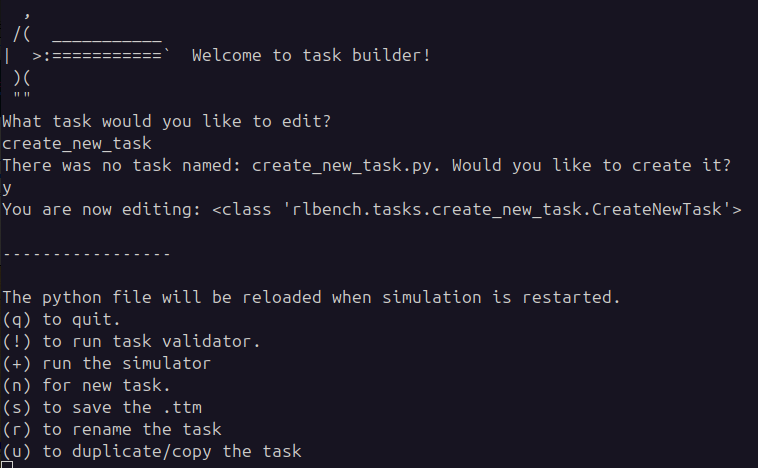
\includegraphics[width=0.8\linewidth]{assets/early-work/task-builder-cli-1.png}      \caption{Task builder CLI: creating a new task}
  \end{subfigure}%
  \hfill
  \begin{subfigure}{0.48\textwidth}
    \centering
    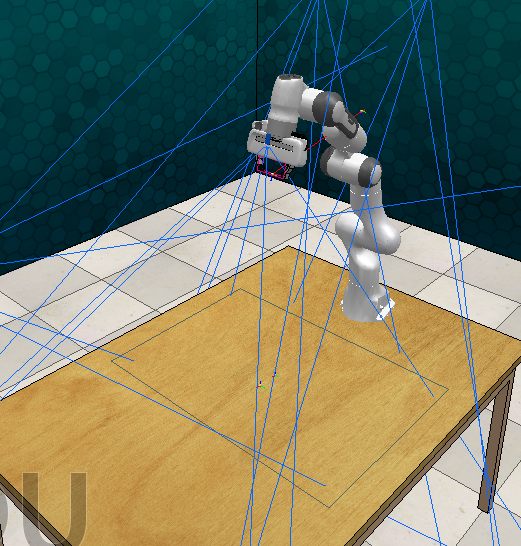
\includegraphics[width=0.8\linewidth]{assets/early-work/task-builder-scene.png}
    \caption{Simulator: Graphical view of the new task}
  \end{subfigure}%
  
  \vspace{0.5cm}
  
  \begin{subfigure}{0.48\linewidth}
    \centering
    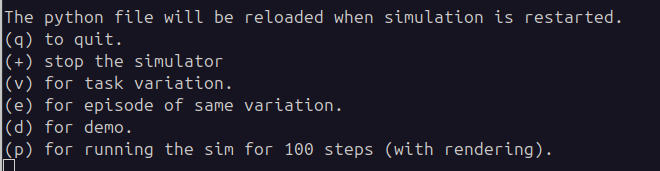
\includegraphics[width=0.8\linewidth]{assets/early-work/task-builder-cli-2.png}
    \caption{Task builder CLI: running the simulator on new task}
  \end{subfigure}
  \hfill
  \begin{subfigure}{0.48\textwidth}
    \centering
    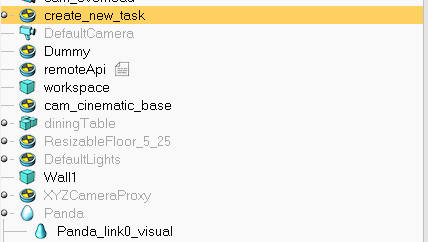
\includegraphics[width=0.8\linewidth]{assets/early-work/task-builder-scene-hierarchy.png}
    \caption{Simulator: Scene Hierarchy of the objects in the new task}
  \end{subfigure}
  \caption{Creating a new task with `task builder'}\label{fig:task-builder}
\end{figure}\todo[color=blue]{reshape, smaller? maybe even move to appendix}


The task I created is simple, see Figure \ref{fig:reach-no-obs}. I decided to use the \emph{Panda arm}, as that seemed to be standard and more importantly immediately supported by RLBench. It has 7 Degrees of Freedom (DoF) and a gripper -so the action space is a 8 dimensional vector. Then a red spherical target, which is not tangible, in the simulation it will be visually rendered but the arm will not collide or interact physically with it. Finally, added a proximity sensor to the target (which is not visually rendered) so the task can be immediately classified as completed by the system.



% //NOTE: relative paths for images, maybe add submodule once project is finished
\begin{figure}[htbp]
  \begin{subfigure}{0.48\linewidth}
    \centering
    \includegraphics[scale=0.4]{../fyp/assets/task-pics/reach-no-obs/random-front.png}      
    \caption{Front View}
  \end{subfigure}%
  \hfill
  \begin{subfigure}{0.48\linewidth}
    \centering
    \includegraphics[scale=0.4]{../fyp/assets/task-pics/reach-no-obs/random-top.png}
    \caption{Top View}
  \end{subfigure}
  \vspace{0.5em}
  \begin{subfigure}{1\linewidth}
    \centering
    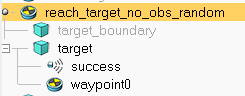
\includegraphics[scale=0.5]{assets/early-work/random-scene-hierarchy.png}
    \caption{Scene Hierarchy}\label{fig:reach-no-obs-hierarchy}
  \end{subfigure}%
  \caption{Reaching Task with no obstacles}\label{fig:reach-no-obs}
\end{figure}

\subsection{Setting up the Environment}
The environment is the all encompassing medium where the simulation happens. The environment contains the information about the scene, the robot: its movement system and control mechanism; information about the observability of the environment in terms of what is available and not available.

I kept my environment all consistent throughout the experimentation. The \verb|action_mode| controls what the stepping action requires as a tuple for the robot to move. I opted for velocity control and arbitrarily decided to apply the gripper movement once the movement was completed. 

This doesn't affect the design of policies in any way, as all the demonstrations were collected in the same environment, and the labelled data will be of this kind. Dataset root points to where to load demonstrations from given a task \ref{subsec:saving-demos}. It can be changed on the same environment when loading a different task. Finally, the observation config, which means what should be recorded and can be later accessible by our root as well as the size of the rgb cameras in terms of pixel resolution. Other cameras and sensors can be enabled and disabled using the \verb|CameraConfig| as shown in Listing \ref{lst:env-setup}; as well as the rest of the launching process.


\begin{listing}[H]
  \begin{minted}[fontsize=\small, bgcolor=gray!10, linenos]{python}

  obs_config = ObservationConfig().set_all(True) 
  enabled_config = CameraConfig(
    rgb=True, depth=False, mask=False, point_cloud=False, image_size=(64, 64)
    render_mode=RenderMode.OPENGL,
  )
  disabled_config = CameraConfig(
    rgb=False, depth=False, mask=False, render_mode=RenderMode.OPENGL)

  obs_config.wrist_camera = enabled_config ## example: enabling a cam/sensor
  obs_config.front_camera = disabled_config

  env = Environment(
    action_mode = MoveArmThenGripper(
      arm_action_mode=JointVelocity(), 
      gripper_action_mode=Discrete()
    ),
    dataset_root = '' if live_demos else 'PATH/TO/YOUR/DATASET',
    obs_config = obs_config, headless = False
  )
  env.launch() ## start the simulator
  \end{minted}
  \caption{Standardised environment launching}\label{lst:env-setup}
\end{listing}

\subsubsection{RLBench Demonstrations}
% NOTE: changed this from being a box, and made an environment section, I think this makes more sense, but review
% \begin{center}
%   \fbox{  
%     \begin{minipage}{\linewidth}
%       \textbf{Aside on RLBench Demonstrations} \par

      Demonstrations are provided encapsulated in a \emph{Demo} class and contain a series of observations (belonging to a class \emph{Observation}). These include state information of the robot and the environment, containing information like the observations of the set cameras and sensors; which need to be configured when the environment is started. This modular approach means I can collect demonstrations, then selectively choose what to use, like ignore a camera or a sensor. \par 
      Demonstrations are created following waypoints. PyRep expects  \emph{Dummy} objects within the scene called ``waypointX'' where sequence number of the waypoint starting from $0$. Then he demonstration engine calculates trajectories to these waypoints in sequence. For example, in Figure \ref{fig:reach-no-obs-hierarchy}, we have `waypoint0' within the target, for which a trajectory will be calculated from the tip of the robot gripper.
%     \end{minipage}
%   }
% \end{center}\todo[color=green]{check centering acts weird sometimes}

By default the demonstrations -which I will refer to as ``demos'' from now on- and specifically the cameras pre-placed in the scene, produce images of resolution $128 \times 128$ pixels. I binned this down to $64 \times 64$. This comes in handy as I can keep the processing power low and can adapt the policy for higher resolution cameras by scaling it up later on. This resolution is an arbitrary choice and might need to increase the scale depending on feature extraction proficiency and whether I can identify this to be a limiting factor to learning a task.

\subsubsection{Saving Demonstrations}\label{subsec:saving-demos}
Final part of the environment is to save demonstrations. To evaluate different policies fairly, I will be needing a way to train them in the same way. So I am planning on controlling the randomisation seed and the fed demos. RLBench provides an interface to save and load demos. However, they do it in an episodic and a slightly convoluted way; for tasks that have clearly defined episodes and variations. I have slightly altered the saving and loading code to easily integrate them into my work. 

I have also recorded all the sensor and all the cameras in these demos, just in case later in the project they are needed. In which case I can just keep using the same demos and keep my findings compatible with earlier results.

